\chapter{Background \& Foundations}\label{chap:k2}
We will have a look at the fundemental requierments required to understanding this work. This will include basic mathematical knowledge - but also more specific ones, to understand the current implementation.
\section{Partial Differential Equations}
Since this paper is about solving partial differential equations (PDEs) with neural networks, it is important to understand what exactly a PDE is. 
We have a D-dimensional spatial domain $\mathcal{X}$, $x = [x_1,x_2,\dots,x_D]^\top \in \mathcal{X}$, and a temporal domain $t\in[0, T]$ (Brandstetter et al., 2021):
\begin{align} &\partial_t u = F(\lambda,t,x,u,\partial_xu,\partial_{xx}u,\dots), && (t,x)\in[0,T]\times \mathbb{X} \\ &u(0,x)=u^0(x),\hspace{2cm}\mathcal{B}[u](t,x)=0 && x\in\mathbb{X}, (t,x)\in[0,T]\times\partial\mathbb{X} \end{align}
We want to know the unique solution $u: [0,T]\times\mathbb{X}\rightarrow\mathbb{R}$ with the initial conditions (IC) $u(0,x)=u^0(x)$ and its boundary conditions $\mathcal{B}[u](t,x)=0$. The PDE parameters are represented by the vector $\lambda = (\lambda_1, \lambda_2,\dots, \lambda_l) \in\mathbb{R}^l$ with $lambda_i\in[a_i, b_i]$ and can influence the underlying system. 
The initial conditions describe the initial state of the system, while the boundary conditions define the PDE at the definition boundaries. 
Both conditions are necessary to obtain a unique solution.
PDEs play an important role in the modern world of physics, for example in the heat equation, which describes how heat is distributed in an area over time:
\[ \lambda\partial_tu=\Delta u \] with $\Delta u = \sum^d_{i=1}\partial_{x^ix^i}u$. 
\section{Active learning}
Before we explain active learning - a subfield of machine learning - 
we have to explain how machine learning itself works. In the words of Ayodele (2010): ``Machine
Learning can still be defined as learning the theory automatically from the data,
through a process of inference, model fitting, or learning from examples''.

But what exactly is ``the data''? There are different strategies how to learn which also define how our machine model 
learns with data, but we will keep our focus on supervised learning. 

In supervised learning, a model is trained on a training data set consisting of input-output pairs. 
The input data represents the information we want the model to learn from or make predictions about, 
while the output data - known as the label - is the expected result for each input.
Although we often use the term ``classification'', labels are not limited to discrete categories. 
If the output is a continuous value, the model is performing regression instead of classification.
From the whole input space, the samples that get added to the training set are chosen at random~\cite{ayodele2010machine}.

In active learning, we try to minimize the amount of training samples we use as input,
while keeping the same/better learning curve. This is done by activley choosing the 
samples for our training set~\cite{ramirez2017active}.
This means we activley query our input data to get it labeled, therefore getting an output value,
by a so called oracle. An oracle is the general term for something that can always label correctly our sample we queried ~\cite{settles2009active}. 
If we train our ensemble, which has multiple neural networks, the approximation for the solution of a sample can differ between the models. There are mainly two factors responsible for this behaviour.
Firstly, the models are using stochastic methods, specifically gradient descent, to approximate solution trajectories, which can lead to different results with the same input. Secondly, the initial weights inside the neural network are stochastically created and are therefore different between models.
The variance between them can give us an indication about 
how informative the sample will be. 
The informativeness therefore called ``uncertainty'' and is modeled via a probabalistic function, with a 
Query-by-Committee algorithm (Seung et al. 1992):
\[
 a_{QbC}(\psi_i):=\frac{1}{N_tN_xN_c}\sum_{j=1}^{N_t}\sum_{k=1}^{N_x}\frac{1}{N_m}\sum_{m=1}^{N_m}\vert\vert\hat{u}_{i,m}(t_j,x_k)- \overline{\hat{u}_i}(t_j, x_k)\vert\vert^2_2
\] 
We have now established a way to define the information content of a sample, but we have yet to explore how samples are actually queried in active learning. Broadly speaking, active learning employs three main strategies, which are illustrated in a simplified manner in Fig.~\ref{fig:AL-overview}.

In pool-based active learning, a collection of samples is first drawn from the input space. The learner then selects specific samples from this pool to query the oracle. In contrast, membership query synthesis (in this work referred to as stochastic query synthesis) bypasses the predefined pool altogether. Instead, the learner queries directly from the input space - or creates completly new unlabeled instances to query.

Finally, in stream-based selective sampling, samples arrive sequentially from the input space. The learner must decide in real-time whether to query the oracle for each incoming sample or discard it. Since the data stream may come from a non-stationary distribution, this approach can sometimes resemble the behavior of query synthesis.
\begin{figure}
    \centering
    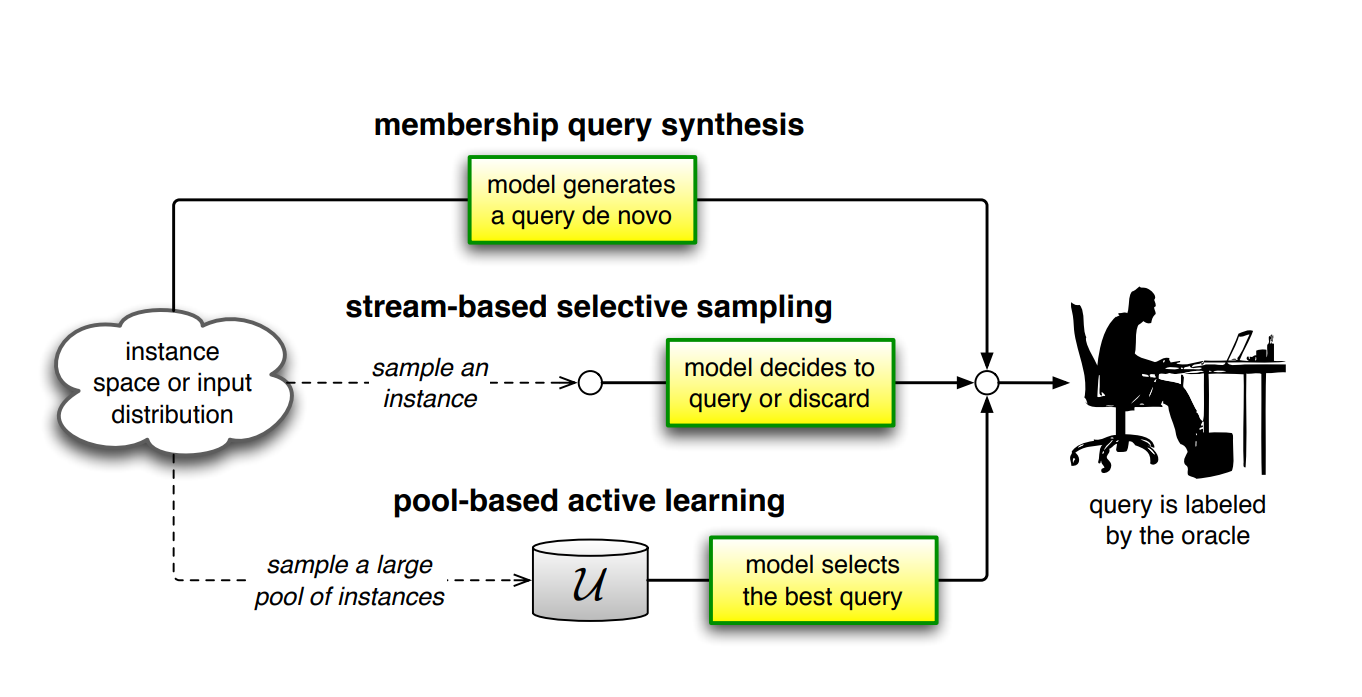
\includegraphics[width=1\linewidth]{../graphics/active_learning.png}
    \caption{The three main methods of active learning by Settels~\cite{settles2009active}}.
    \label{fig:AL-overview}
\end{figure}
\subsection{Pool-Based active learning}
The pool-based approach is about sampling a large pool 
of unlabeled instances from the original instance 
space/input distribution. Samples from this pool then 
get queried to an oracle which will generate a label, 
visualized in Fig. ~\ref{fig:AL-pool}.

\begin{figure}[t!]
    \centering
    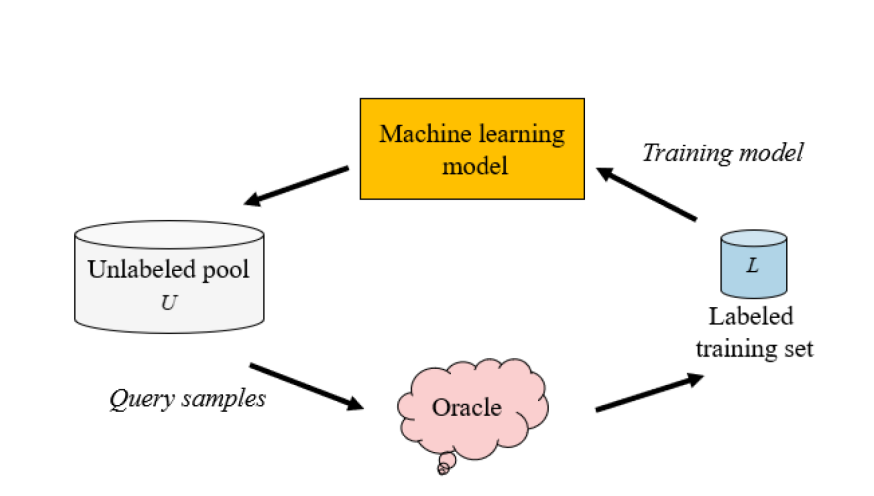
\includegraphics[width=1\linewidth]{../graphics/pool-based.png}
    \caption{The pool-based cycle done by Ren et al.~\cite{ren2021survey}}
    \label{fig:AL-pool}
\end{figure}

In mathematical terms, we will reuse the 
definition from Ren et al.~\cite{ren2021survey}. 
Let $U^n = \{\X, \Y\}$ be the unlabeled dataset with n samples,
with $\X$ being the sample size and $\Y$ being the label size.
P(x,y) is a potential distribution, with $x \in \X$, $y \in \Y$. 
It represents the joint probability distribution of the sample 
$x$ and the label $y$. $L^m=\{X,Y\}$ is the training set with m labeled instances. 
In our case, the input space includes both ICs and PDE parameters for a given PDE, each taking continuous values. 
As a result, the input space is effectively infinite and our pool is created by sampling a finite amount of samples.

Now the goal is to create a query strategy Q that queries samples from $U^n$ to be labeled by the oracle: $U^n \xrightarrow{\text{Q}} L^m$. 
We therefore have to choose which samples from we want to pass to the numerical solver and add to the training set.
Here we can use the uncertainty as an indicator of the informativeness of the samples to select the samples.
This approach is easy to implement and often improves on random sampling. It is the most common approach~\cite{zhan2021comparative}. 
In the context of deep active learning, the combination of deep learning and active learning, 
single-sample-based methods reach their limits as single points do not have a statistically 
significant impact. Furthermore, training on individual samples requires a full iteration of the deep learning network for each one, which is computationally expensive. To mitigate this, rather than querying single entities, it is more efficient to process an entire batch at once~\cite{sener2017active}.
\subsection{Batch active learning}
When training a deep-learning network with a pool-based approach, 
it is inefficient to query single points. 
In batch active learning, instead of a single point, 
a whole batch of size $K$ with $K\in\mathbb{N}$  
is selected from the given pool~\cite{ren2021survey}. 
The batch of unlabeled data 
$\mathcal{B} = \{x_1,x_2,...,x_b\}\subseteq U$ 
is selected based on an acquisition function $a$.
One common method how to generate a batch is to query the $K$ samples with the highest uncertainty, also known as Top-$K$.
The uncertainty is thereby evaluated at each sample inside the pool.
\[
a_s^{\text{batch}}(\mathcal{I}^{\text{train}};K) := arg\,max_{I\subseteq\mathcal{I}^{\text{pool}},\lvert I\rvert = K}\sum_{i\in I}s(i;\mathcal{I}^{\text{train}})
\]    
with $a$ being the acquisition function, 
$\mathcal{I}^{\text{train}}$ being the indices of the samples 
in the training data set and $\mathcal{I}^{\text{pool}}$ being the indices 
of the samples in the pool data set~\cite{kirsch2021stochastic}.
\subsection{Stochastic batch active learning}
Selecting the Top-$K$ instances can lack diversity, therefore
Kirsch et al.~\cite{kirsch2021stochastic} introduced stochastic batch 
active learning (SBAL). SBAL samples without replacement the input 
$\psi$ from the pool $S_{\text{pool}}$ with the probability distribution 
\[p_{\text{power}(\psi)}\propto\alpha(\psi)^m\cdot p_{pool}(\psi)\] 
with $m$ being a 
hyperparameter, that is controlling the sharpness of the distribution. Since the pool is uniformly sampled, $p_{pool}(\psi)$ is equal to one and cancels out.



\subsection{Query synthesis active learning}
Creating and evaluating the pool can be quite costly, especially if the pool size is set too large. To avoid 
this problem, another active learning method ``Query synthesis'' was introduced~\cite{Angluin1988}. 
Query synthesis samples to the oracle directly from the input space or can even create new samples to query~\cite{wang2015active}.

For us this means to query samples directly to the numerical solver, which can be a great advantage for us. Utilizing the uncertainty, we can potentially sample from regions with higher uncertainties than it would be possible for pool-based methods  - since we are not bound to a specific fixed amount of samples. One advantage for us is the ability to calculate the gradient of the uncertainty, which allowes us to sample from regions with the highest uncertainty.

The challenge here is to choose a fitting algorithm, defining the 
query strategy. 
We will choose an implementation of Markov chain Monte Carlo.


